\graphicspath{{./figures/}}
\section{Development of the solution}
\glsadd{dfg}\glsadd{cgra}\glsadd{pe}\glsadd{dag}\glsadd{sat}\glsadd{smt}\glsadd{z3}\glsadd{alu}\glsadd{oneshot}\glsadd{mapping}\glsadd{mapper}\glsadd{lisagnn}\glsadd{gnn}\glsadd{json}\glsadd{label0}\glsadd{ai}\glsadd{satmink}\glsadd{graphsage}

\subsection{Requirements and constraints}
As a research project, the requirements were deliberately open-ended. The main goal was to investigate how AI could guide DFG-to-CGRA mapping and deliver a working prototype that could be evaluated within one semester.

Throughout the internship, requirements and constraints constantly evolved. The final prototype was shaped by the following needs and restrictions:
\begin{itemize}
    \item \textbf{Research-team goal:} Use learned information to improve a mapping decision.
    \item \textbf{Integration need:} Accept and produce stable JSON so the parallel code-generation project could consume the resulting mappings.
    \item \textbf{Functional need:} Accept a DFG and CGRA description, split graphs that do not fit in one configuration, validate every partition, and export PE assignments and operand connections.
    \item \textbf{Quality goal:} Reduce inter-partition cuts without making mapping time impractical, because every cut implies an additional value transfer.
    \item \textbf{Validation goal:} Compare the learned approach with exhaustive and heuristic alternatives using repeatable experiments.
\end{itemize}

Due to time constraints, the complexity of the problem, and the scope of the internship, some simplifications were assumed about how the CGRA and DFG were represented and processed, which do not reflect the full complexity of the real-world scenario. One-shot spatial mapping was assumed for each partition, internal dependencies required direct neighboring PEs, and cross-partition values were represented through synthetic memory operations. Our model assumes that the CGRA has a clock period long enough for every supported operation to complete in one clock cycle. Additionally, the DFG's cut edges are represented as injected memory operations, which are not part of the original DFG\@. Finally, the DFG itself is assumed to be a directed acyclic graph, which is not always the case in real-world applications, representing a loop that is unrolled. The proposed flow does not do modulo scheduling nor does it determine a kernel; the whole DFG is assumed to be a single kernel.

\begin{figure}[t!]
    \centering
    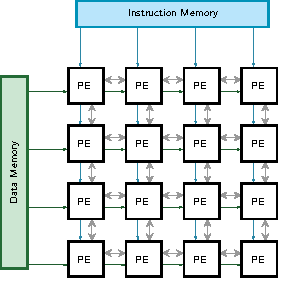
\includegraphics[width=0.35\linewidth]{output-figure0.pdf}
    \caption{Targeted $4\times4$ homogeneous CGRA: 16 PEs with full ALU capability and memory access, with nearest-neighbour connections.}
    \label{fig:cgra_arch}
\end{figure}

The targeted CGRA for the final experiments was a homogeneous $4\times4$ array (Figure~\ref{fig:cgra_arch}), and the DFGs were synthetic, generated from small kernel templates.




% DRAFTING SUGGESTION:
% Present the requirements as needs discovered during the internship, not as a
% formal description of the paper's method. Explain that the initial brief was
% deliberately open: investigate how AI could guide DFG-to-CGRA mapping and
% deliver a working prototype that could be evaluated within one semester.
%
% Separate the requirements by source:
% - Research-team goal: use learned information to improve a mapping decision.
% - Integration need raised in meetings: accept and produce stable JSON so the
%   parallel code-generation project could consume the resulting mappings.
% - Functional need: accept a DFG and CGRA description, split graphs that do
%   not fit in one configuration, validate every partition, and export PE
%   assignments and operand connections.
% - Quality goal: reduce inter-partition cuts without making mapping time
%   impractical, because every cut implies an additional value transfer.
% - Validation goal: compare the learned approach with exact and heuristic
%   alternatives using repeatable experiments.
%
% Then state the restrictions that shaped the delivered prototype. The mapper
% validates spatial placement only; each partition is treated as a one-shot
% configuration, internal dependencies require direct neighbouring PEs, and
% cross-partition values are represented through synthetic memory operations.
% The final experiments target a homogeneous 4 x 4 CGRA and synthetic DFGs.
% Clarify that these restrictions were conscious scope decisions made after the
% LISA/SAT-MapIt integration difficulties described in the meeting history.

\subsection{Architecture and technologies}

\begin{figure}[t!]
    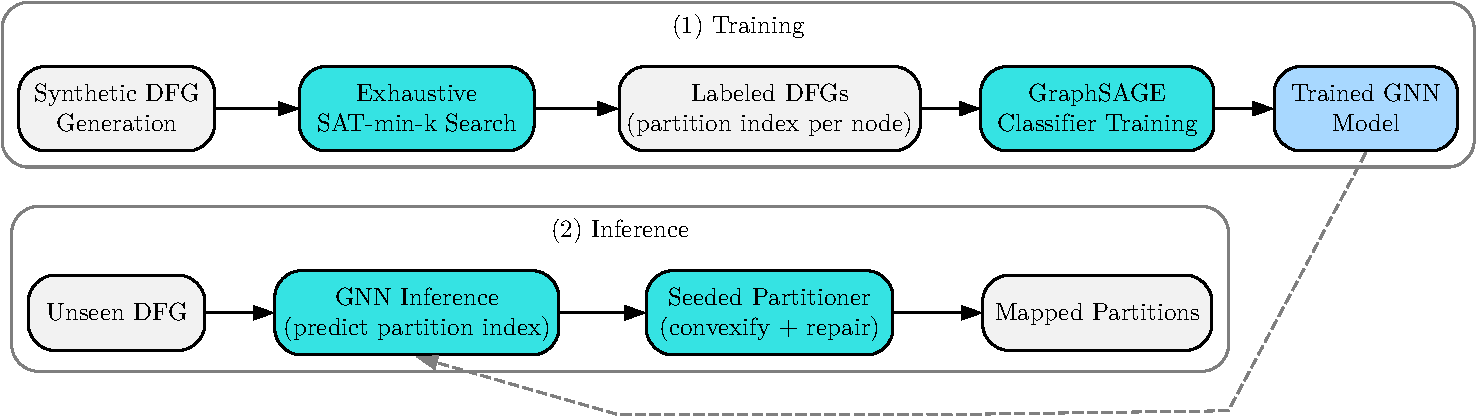
\includegraphics[width=\textwidth]{flow-crop.pdf}
    \caption{Overview of the proposed flow. The methodology is divided into two distinct phases: training the GNN and inference-time graph partitioning with SAT-based spatial validation.}
    \label{fig:flow}
\end{figure}

The final framework is illustrated in Figure~\ref{fig:flow}. The flow can be divided into two parts, the training phase and the inference phase. The training phase is responsible for generating synthetic DFGs, producing ground-truth labels with the exhaustive partitioner and mapper, and training the GNN model. The inference phase uses the trained GNN to predict partitions for new DFGs, which are then fed as seeds to the topology-aware mapper, which repairs infeasible predictions and validates the final partitions with the SAT mapper.

Technology-wise, the tool was developed in Python, which allowed fast experimentation and integration of graph, machine-learning and solver components, and has been the choice for this problem by the state of the art. The \gls{z3} \gls{smt} solver was used to express and check placement constraints. GitLab was used for version control, and the actual graph/ML libraries used in the implementation were PyTorch Geometric for GNN training and inference, and NumPy for numerical operations.

% DRAFTING SUGGESTION:
% Introduce the architecture from the perspective of how the work was organised
% and why each component was needed. A useful opening is to distinguish an
% offline preparation phase from the inference-time mapping flow:
%
% 1. Generate varied DFGs from small kernel templates.
% 2. Search for high-quality feasible partitions with the exhaustive SAT-min-k
%    process and use them as supervised labels.
% 3. Train a GraphSAGE model to predict a partition index for each DFG node.
% 4. At inference time, repair those predictions into ordered, feasible
%    partitions and validate their spatial placement with the SAT mapper.
% 5. Export the validated mappings in the agreed JSON format.
%
% Explain the technology choices in relation to internship needs. Mention
% Python for fast experimentation and integration of graph, machine-learning
% and solver components; Z3 for expressing and checking placement constraints;
% GitLab for version control; and the actual graph/ML libraries used in the
% implementation. State why a custom spatial SAT mapper was implemented rather
% than reproducing SAT-MapIt's complete modulo-scheduling flow.
%
% Suggested figure: retain a simplified pipeline diagram, but describe it as
% the architecture that emerged through iteration rather than reproducing the
% paper's proposed-approach narrative.

\subsubsection{Evolution of the technical approach}

As has already been introduced by the sequence of meetings, the technical approach evolved through several iterations. After reaching the final idea for the flow (partitioning large graphs, training a model to predict partitions, then running a heuristic SAT-based mapper to validate the partitions), the next step was to evolve the technical approach. The first advancement was implementing the exhaustive \gls{satmink} algorithm, which allowed us to produce better ground-truth labels to improve the GNN's predictions. By implementing the pure greedy (list-scheduling) approach with the GNN-guided priorities, we concluded that the success rate was too low, and that the only successes were on simple graphs, which did not stress the routing constraints of the CGRA\@. Investigating the failures, we concluded that the GNN predictions were not enough to guarantee a feasible mapping, and that a repair step was needed. The repair step was implemented as a topology-aware partitioner that would split infeasible partitions at a feasible topological boundary until all partitions were feasible. For later evaluation we also implemented a pure raw GNN approach that would just take the GNN predictions and run the SAT-based mapper on them, without any repair step. Although this now becomes an iterative approach, with the GNN predictions the topology-aware partitioner is able to produce feasible partitions with low iteration counts, later presented in the results section.

% DRAFTING SUGGESTION:
% Use this subsection to connect the meeting history to the final architecture.
% Describe the sequence of decisions: reproduce and study LISA; investigate
% SAT-MapIt and NaviMap; discard NaviMap because its implementation and
% training cost did not fit the available time; identify incompatibilities
% between LISA labels and SAT-MapIt's temporal model; and reformulate the work
% around partitioning followed by one-shot spatial mapping.
%
% This is one of the main differences from the paper. The report should make
% the unsuccessful paths and trade-offs visible because they demonstrate
% problem analysis, autonomy and engineering judgement. Explain what was
% learned from each discarded direction and how it affected the next
% implementation step.

\subsubsection{DFG representation and synthetic data generation}

To train neural networks, a large number of labelled examples is needed. Similar to what the LISA~\cite{lisa2022} approach does, we implemented a synthetic DFG generator capable of producing a large number of DFGs. Our generator, in contrast to the LISA generator which is purely stochastic, is based on a set of seed templates, which are then mutated, with tunable parameters, to produce a large number of DFGs. The two seed templates are based on the inner loop body of a matrix multiplication and convolution. The mutations are divided into three families: depth mutations, breadth mutations and neutral mutations. Depth mutations increase the length of dependency chains, breadth mutations increase the number of parallel operations and routing pressure, and neutral mutations diversify the operations without changing the topology.

\begin{figure}[!t]
    \centering
    \begin{subfigure}[t]{0.46\textwidth}
        \centering
        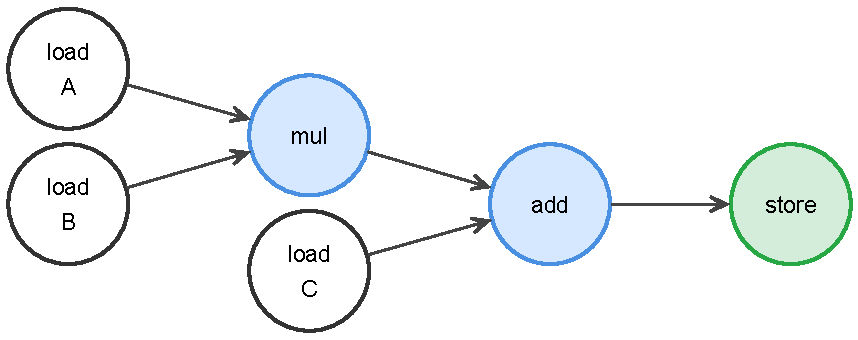
\includegraphics[width=\textwidth]{matmaul_template.pdf}
        \caption{Matmul kernel template}
        \label{fig:matmul_dfg}
    \end{subfigure}
    \hfill
    \begin{subfigure}[t]{0.49\textwidth}
        \centering
        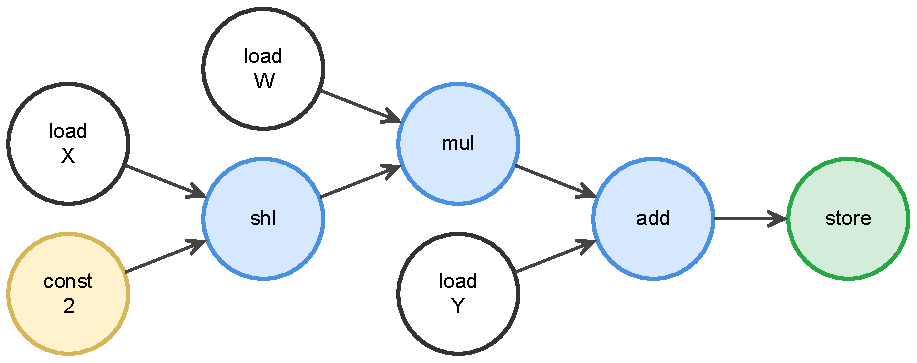
\includegraphics[width=\textwidth]{conv.pdf}
        \caption{Convolution kernel template}
        \label{fig:conv_dfg}
    \end{subfigure}
    
    \caption{Kernel templates used as a base for DFG generation.}
    \label{fig:kernel_templates}
\end{figure}



% DRAFTING SUGGESTION:
% Describe the implementation work needed before any learned mapping could be
% tested. Explain how the common JSON representation was defined for
% instruction nodes, constants, loads, stores, metadata and dependency edges,
% and how that representation reduced friction between generator, partitioner,
% mapper and code generation.
%
% Explain why a synthetic generator was necessary: the project needed enough
% labelled graphs for training and evaluation, while compiler-extracted
% examples were limited and the original LISA flow was too slow to reproduce at
% the required scale. Describe the matrix-multiplication and convolution seed
% templates, then explain the three mutation families in practical terms:
% depth mutations lengthened dependency chains, breadth mutations created more
% parallel work and routing pressure, and neutral mutations diversified
% operations without changing topology.
%
% Include representative before/after graph screenshots or diagrams. Focus the
% text on what you implemented, which invariants the generator had to preserve,
% and which generation errors or unrealistic cases had to be filtered.

\subsubsection{SAT-based mapper and ground-truth generation}

The SAT-based mapper that was implemented is a simplified version of the SAT-MapIt~\cite{satmapit2023} mapper that only performs one-shot spatial mapping. The mapper receives a DFG and a CGRA description, and for each instruction, it chooses exactly one compatible PE\@. No PE may host more than one instruction, dependent instructions must be placed on connected PEs, and memory operations must use memory-capable PEs when the architecture is heterogeneous. If the Z3 solver can find a valid assignment, the mapper returns the mapping; otherwise, it returns an infeasible result.

Ground-truth generation for the GNN training was performed by the \gls{satmink} algorithm, which is an exhaustive search for the minimum number of partitions needed to map a DFG\@. Starting from the minimum partition count based on CGRA capacity, the implementation enumerates ordered candidate assignments, rejects candidates that violate cheap structural checks, and SAT-validates the remaining partitions. After finding all feasible partitions, the one with the minimum partition count and edge cuts is selected as the ground-truth label. To control the quality of the output, parameters such as early stop on zero cut edges and maximum partition count are configurable.

% DRAFTING SUGGESTION:
% Explain the custom SAT mapper as a validation tool developed during the
% internship. For each instruction, the solver chooses exactly one compatible
% PE; no PE may host more than one instruction; dependent instructions must be
% placed on connected PEs; and memory operations must use memory-capable PEs
% when the architecture is heterogeneous. Mention any additional resource
% checks performed after a model is returned.
%
% Describe how this mapper enabled SAT-min-k ground-truth generation. Starting
% from the minimum partition count implied by capacity, the implementation
% enumerates ordered candidate assignments, materialises cross-partition
% dependencies, rejects candidates that violate cheap structural checks, and
% SAT-validates the remaining partitions. The selected label minimises the
% partition count first and edge cuts second.
%
% Do not reproduce the complete mathematical formulation or algorithm listing
% from the paper. Instead, explain the development effort, the reason for each
% check, and the practical scalability problem observed when exhaustive search
% was applied to larger or wider graphs. Include one small worked example that
% follows a graph from candidate split to accepted or rejected mapping.

\subsubsection{GNN training and inference}

The GNN model used in this work is a \gls{graphsage}~\cite{hamilton2017inductive} classifier that receives per-node structural and operation features, the same ones used in LISA~\cite{lisa2022}, and predicts the partition index learned from \gls{satmink} solutions. The model was trained on 1500 synthetic DFGs. The dataset was biased toward moderate graph sizes and low-to-medium parallelism to ensure that the \gls{satmink} algorithm could produce ground-truth labels in a reasonable time. This choice means that the model may not generalize well to larger or more complex graphs.

During inference time, the GNN predicts partition indices for each node in an unseen DFG\@. The predictions are then passed as seeds to the topology-aware partitioner, which repairs infeasible predictions and produces valid partitions for SAT-based spatial validation.

% DRAFTING SUGGESTION:
% Describe the machine-learning work as an attempt to approximate the expensive
% ground-truth search. State that the GraphSAGE classifier receives per-node
% structural and operation features and predicts the partition index learned
% from SAT-min-k solutions. Explain how variable graph sizes and imbalanced
% partition labels affected dataset preparation, batching, loss selection and
% evaluation.
%
% Retain the relevant experimental detail: 1650 synthetic DFGs were generated,
% with 1500 used for training/ground-truth production and 150 held out for the
% final comparison. Explain why the dataset was biased toward moderate graph
% sizes and low-to-medium parallelism, and acknowledge what this choice means
% for generalisation.
%
% Include the concrete training workflow, configuration and stopping criteria
% used in the repository, plus any failed training attempts or changes that
% materially improved predictions. Avoid presenting the GNN as a black box or
% copying the paper's loss equation without discussing how it was applied.

\subsubsection{Prediction repair and dependency representation}

In an ideal scenario, the GNN is able to predict feasible partitions for any DFG\@. However, in practice, and with the limited time and computational resources available during training, the GNN was not able to learn a perfect mapping. As such, the predicted partitions may violate dependency order, exceed resource capacity, or fail spatial SAT validation. To address this, a topology-aware partitioner was implemented to repair the predicted partitions. The repair process first makes partition indices consistent with the DFG topology and compacts empty indices, enforcing that a consumer node cannot be placed before its producers. Then it tests each partition and splits infeasible ones at a feasible topological boundary until all remaining partitions can be mapped.

As mentioned before, cut edges are represented as synthetic store/load operations, which are injected into the DFG and are part of the mapping. This was the way the team decided to represent cross-partition dependencies, so that each partition becomes self-contained for one-shot mapping. The original edge is replaced by a store operation in the producer partition and a load operation in the consumer partition, which are connected to the same memory location. This way, the mapper can treat each partition independently, while still preserving the data flow between them. 

% DRAFTING SUGGESTION:
% Explain why raw GNN output could not be trusted directly: a predicted split
% may violate dependency order, exceed resource capacity, or fail spatial SAT
% validation. Describe the repair process in implementation order. First make
% partition indices consistent with the DFG topology and compact empty
% indices. Then test partitions and split infeasible ones at a feasible
% topological boundary until all remaining partitions can be mapped.
%
% Describe how dependencies crossing a partition boundary are rewritten as
% synthetic store/load operations so that each partition becomes self-contained
% for one-shot mapping. Include a small diagram showing the original edge, the
% partition boundary and the materialised memory operations.
%
% Discuss the trade-off exposed by this component: repair substantially
% improves feasibility, but every additional split can increase communication
% overhead. This motivates measuring both success rate and edge cuts.

\subsection{Developed solution}

The final solution is a complete pipeline that takes a DFG and a CGRA description, generates annotations that are fed into the GNN which predicts partitions, repairs infeasible predictions, and validates the final partitions with a SAT-based mapper. The output is a set of valid partitions with PE assignments and operand connections, exported in JSON format for use in the code generation project.

% DRAFTING SUGGESTION:
% Present the final prototype as someone using or integrating it would
% experience it. Walk through one realistic end-to-end execution:
%
% 1. Select or generate a JSON DFG and a target CGRA description.
% 2. Run GNN inference to annotate nodes with suggested partitions.
% 3. Repair and materialise the partitions.
% 4. SAT-map each partition to the CGRA.
% 5. Inspect the exported per-partition JSON mappings consumed by the
%    code-generation work.
%
% Add screenshots or excerpts of the input graph, predicted partitioning,
% repaired partitioning and final PE placement. Explain the most important
% output fields and how errors are reported when a graph cannot be processed.
% Name the final deliverables produced during the internship: generator,
% shared data representation, SAT mapper, exact labelling process, trained GNN,
% guided partitioner, benchmark scripts/results and scientific paper.

\subsection{Validation}

\subsubsection{Validation strategy and experimental setup}

\begin{table}[!t]
\footnotesize
\centering
\caption{Structural statistics of the training (1500 graphs) and evaluation 
(150 graphs) dataset splits. All values reported as mean $\pm$ std 
(min--max).}
\label{tab:dataset_stats}
\setlength{\tabcolsep}{4pt}
\begin{tabular}{lrr}
\textbf{Metric} & \textbf{Training} & \textbf{Evaluation} \\
\midrule
Nodes           & $22.51 \pm 3.31$ \ (16--28) & $23.16 \pm 2.92$ \ (16--28) \\
Edges           & $21.77 \pm 3.39$ \ (15--29) & $22.45 \pm 2.97$ \ (15--28) \\
Depth           & $8.19 \pm 1.32$ \ (6--13)   & $8.40 \pm 1.30$ \ (6--12)   \\
Parallelism     & $4.26 \pm 0.95$ \ (2--8)    & $4.19 \pm 0.97$ \ (2--7)    \\
Instr-Level Parallelism             & $2.21 \pm 0.45$ \ (1.3--4.0) & $2.21 \pm 0.48$ \ (1.3--3.8) \\
Memory ratio    & $0.42 \pm 0.07$ \ (0.21--0.62) & $0.42 \pm 0.08$ \ (0.25--0.60) \\
\bottomrule
\end{tabular}
\end{table}


To evaluate the proposed solution, a $4\times4$ homogeneous CGRA (Figure~\ref{fig:cgra_arch}) was targeted. A total of 1650 DFGs were generated, with 1500 used for training and ground-truth generation, and 150 held out for the final evaluation. The graph characteristics are described in Table~\ref{tab:dataset_stats}.

The evaluation compared five strategies: SAT-min-k, Greedy, Topological, GNN-raw, and GNN-guided. 
\gls{satmink} is the exhaustive search for the minimum number of partitions, which serves as a ground-truth reference. Greedy is a simple list-scheduling baseline that maps nodes in topological order without any learned guidance. Topological is the repair-only strategy that uses the topology-aware partitioner to fix infeasible predictions. GNN-raw is the GNN prediction without any repair, and GNN-guided combines the GNN predictions with the repair step.

% DRAFTING SUGGESTION:
% Tie validation explicitly back to the requirements. Explain which checks
% establish functional correctness, which experiments assess partition
% quality, and which measurements assess practical runtime. Mention unit or
% end-to-end tests used during development if available, in addition to the
% final benchmark.
%
% Describe the held-out benchmark of 150 synthetic DFGs and the homogeneous
% 4 x 4 CGRA. Introduce the five compared strategies by the question each one
% answers:
% - SAT-min-k: how good can a feasible partition be with exhaustive search?
% - Greedy: what happens with a cheap irreversible baseline?
% - Topological: how much does repair achieve without learned guidance?
% - GNN-raw: how useful are predictions without repair?
% - GNN-guided: what is achieved when prediction and repair are combined?
%
% Explain why a second comparison restricted to the 106 graphs solved by
% GNN-raw is necessary. It removes selection bias and makes the raw-versus-
% repaired quality comparison fair.

\subsubsection{Results and interpretation}

\begin{table}[!t]
\centering
\caption{Benchmark results. (a)~full 150-graph evaluation set; (b)~restricted to
the 106 graphs solved by \textsc{GNN-raw}, the like-for-like subset for the
\textsc{GNN-raw} vs.\ \textsc{GNN-guided} comparison. $\dagger$~Greedy results are
reported on its successes only (23 in (a), 20 in (b)) and are not directly comparable.}
\label{tab:benchmark}

\begin{subtable}{\linewidth}
\centering
\caption{Full 150-graph evaluation set.}
\label{tab:benchmark_results}
\resizebox{\linewidth}{!}{%
\begin{tabular}{lrrrrr}
& \textsc{SAT-min-k} & Greedy & Topological & \textsc{GNN-raw} & \textsc{GNN-guided} \\
\midrule
Success rate
    & $100\%$ & $15.3\%$ & $92.7\%$ & $70.7\%$ & $98.0\%$ \\
\midrule
Mean edge cuts
    & $1.31 \pm 0.09$ & $1.52 \pm 0.37^\dagger$ & $3.22 \pm 0.25$ & $1.74 \pm 0.17$ & $2.15 \pm 0.20$ \\
\midrule
Partitioning (s)
    & $0.581 \pm 0.396$ & $0.005 \pm 0.001$ & $0.007 \pm 0.001$ & $0.0004 \pm 0.00001$ & $0.004 \pm 0.0004$ \\
SAT mapping (s)
    & $11.508 \pm 2.276$ & $0.071 \pm 0.004$ & $0.498 \pm 0.047$ & $0.071 \pm 0.002$ & $0.243 \pm 0.039$ \\
SAT checks / part.
    & $80.59 \pm 12.40$ & $1.00 \pm 0.00$ & $3.71 \pm 0.21$ & $1.00 \pm 0.00$ & $2.36 \pm 0.11$ \\
\bottomrule
\end{tabular}}
\end{subtable}

\vspace{1.5ex}

\begin{subtable}{\linewidth}
\centering
\caption{106-graph subset solved by \textsc{GNN-raw}.}
\label{tab:benchmark_common}
\resizebox{\linewidth}{!}{%
\begin{tabular}{lrrrrr}
& \textsc{SAT-min-k} & Greedy & Topological & \textsc{GNN-raw} & \textsc{GNN-guided} \\
\midrule
Success rate
    & $100\%$ & $18.9\%$ & $94.3\%$ & $100\%$ & $100\%$ \\
\midrule
Mean edge cuts
    & $1.09 \pm 0.06$ & $1.55 \pm 0.41^\dagger$ & $3.00 \pm 0.29$ & $1.74 \pm 0.17$ & $1.60 \pm 0.17$ \\
\midrule
Partitioning (s)
    & $0.089 \pm 0.013$ & $0.005 \pm 0.001$ & $0.005 \pm 0.0005$ & $0.0003 \pm 0.00001$ & $0.002 \pm 0.0001$ \\
SAT mapping (s)
    & $7.923 \pm 1.265$ & $0.061 \pm 0.004$ & $0.393 \pm 0.044$ & $0.060 \pm 0.002$ & $0.133 \pm 0.028$ \\
SAT checks / part.
    & $70.44 \pm 8.87$ & $1.00 \pm 0.00$ & $3.60 \pm 0.24$ & $1.00 \pm 0.00$ & $2.01 \pm 0.02$ \\
\bottomrule
\end{tabular}}
\end{subtable}

\vspace{1ex}
\begin{minipage}{\linewidth}
\scriptsize
\textbf{Strategies.}
\textsc{SAT-min-k}: exhaustive search over partition assignments; optimal reference. Greedy: single-pass list scheduling, no repair (fast baseline). Topological: topology-aware partitioner with all nodes seeded to one partition; feasibility repair only.
\textsc{GNN-raw}: raw GNN predictions submitted directly, without feasibility checks or repair.
\textsc{GNN-guided}: topology-aware partitioner seeded with GNN predictions (proposed method).
\end{minipage}
\end{table}

Tables~\ref{tab:benchmark_results} and~\ref{tab:benchmark_common} summarise the benchmark results. On the full 150-graph evaluation set, the greedy baseline mapped only 23 graphs ($15.3$\%), while GNN-raw mapped 106 graphs ($70.7$\%), the topology-only repair mapped 139 graphs ($92.7$\%), and GNN-guided mapped 147 graphs ($98.0$\%). The mean edge cuts for the full set were $3.22$ for the unguided topological method, $2.15$ for GNN-guided, and $1.31$ for SAT-min-k. On this set, the GNN-raw approach seemed to show a slight improvement over the topological method, with $1.74$ mean cuts. To evaluate this improvement fairly, we restricted the comparison to the 106 graphs that GNN-raw could map in Table~\ref{tab:benchmark_common}. On this subset, GNN-guided achieved $1.60$ mean cuts versus $1.74$ for GNN-raw and $1.09$ for SAT-min-k. This shows that on the same set of graphs, the GNN-guided approach improves the learned split, and not just feasibility.

Regarding runtime, GNN-raw is the overall fastest strategy, partitioning takes $0.4$\,ms and SAT mapping $0.07$\,s, matching greedy's per-partition cost since both submit exactly one SAT check per partition. GNN-guided (partitioning $4$\,ms, SAT mapping $0.24$\,s) is approximately $50\times$ faster end-to-end than SAT-min-k ($12.1$\,s total), while the topological strategy ($0.50$\,s SAT mapping) is slower than \textsc{GNN-guided} despite producing worse partitions, because a poor seed drives more feasibility-repair iterations and consequently more SAT checks per partition.

% DRAFTING SUGGESTION:
% Report the key results, but frame them as evidence about the engineering
% decisions made during the internship rather than as a compressed paper
% results section.
%
% Important values to retain:
% - The greedy baseline mapped 23/150 graphs (15.3%).
% - GNN-raw mapped 106/150 graphs (70.7%).
% - The topology-only repair mapped 139/150 graphs (92.7%).
% - GNN-guided mapped 147/150 graphs (98.0%).
% - On the full set, GNN-guided reduced mean cuts from 3.22 for the unguided
%   topological method to 2.15, while SAT-min-k achieved 1.31.
% - On the fair 106-graph subset, GNN-guided achieved 1.60 mean cuts versus
%   1.74 for GNN-raw and 1.09 for SAT-min-k.
% - GNN-guided required about 0.25 seconds per graph end-to-end, around
%   50 times less than SAT-min-k at roughly 12.1 seconds.
%
% Interpret each group of values. The success rates show that repair is needed
% for dependable mappings. The common-subset cut counts show that repair does
% not merely restore feasibility; it also improves the learned split. Runtime
% demonstrates why exhaustive ground-truth generation is suitable offline but
% not as the normal mapping strategy.
%
% Include the full tables if page limits allow, but follow each table with a
% short discussion of what requirement it validates and what conclusion can
% legitimately be drawn. Do not compare greedy cut quality directly with
% methods evaluated on almost the full set, because greedy succeeds only on a
% small and easier subset.

\section{Conclusions}
\glsadd{cgra}

\subsection{Results achieved and individual contribution}

Overall, I have successfully implemented a complete pipeline for DFG-to-CGRA mapping guided by a learned model. The work progressed from state-of-the-art study to a complete experimental prototype combining data generation, exact labelling, learned prediction, repair and SAT-based spatial validation. The central result is that learned guidance improved the feasibility and cut quality of the practical partitioner while remaining much faster than exhaustive search.

The INForum 2026 paper is a project outcome, it communicates the research contribution and presents the results, whereas this report documents the complete internship process and my individual work. The Capstone Project was carried out individually in a team setting: I implemented and evaluated the mapping pipeline and wrote this report. Francisco developed the separate downstream code-generation project, while the supervisors guided technical decisions, reviewed results and co-authored/reviewed the scientific paper.

% DRAFTING SUGGESTION:
% Summarise the internship against its original goals. State that the work
% progressed from state-of-the-art study to a complete experimental prototype
% combining data generation, exact labelling, learned prediction, repair and
% SAT-based spatial validation. Emphasise the central result: learned guidance
% improved the feasibility and cut quality of the practical partitioner while
% remaining much faster than exhaustive search.
%
% Clarify individual contribution precisely. The Capstone Project was carried
% out individually: you implemented and evaluated the mapping pipeline and
% wrote this report. Francisco developed the separate downstream code-generation
% project, while the supervisors guided technical decisions, reviewed results
% and co-authored/reviewed the scientific paper. If the course requires a
% percentage, agree the wording and number with the tutors before inserting it.
%
% Mention the INForum 2026 paper as a project outcome, but explain that the
% paper communicates the research contribution whereas this report documents
% the complete internship process and your individual work.

\subsection{Lessons learned}

This internship has been a valuable learning experience, both technically and professionally. On the technical side, I gained experience in neural networks, graph neural networks, graph theory, accelerator architectures, and SAT solvers. The biggest takeaway for me was the importance of reading the state of the art. I learned how to search for papers, read them, and extract the relevant information to apply it to my own work. I also learned how to design and implement a complete pipeline for a complex problem, from data generation to model training and evaluation.

Working in a research team has also taught me valuable professional skills. I learned how to work autonomously on an open-ended research task, how to prepare concise weekly presentations, and how to receive and act on critical feedback.

% DRAFTING SUGGESTION:
% Reflect on both technical and behavioural learning. Technical lessons can
% include modelling a hardware-mapping problem as constraints, using exact
% solvers to produce supervision for a learned approximation, handling graph
% data, designing fair experiments, and recognising selection bias in result
% comparisons.
%
% For professional skills, discuss working autonomously in an open-ended
% research task, preparing concise weekly presentations, receiving and acting
% on critical feedback, coordinating a stable interface with a parallel
% project, and repeatedly reducing scope without losing the core research
% question. Use one or two concrete examples from the meeting history rather
% than making only general claims.

\subsection{Limitations and future work}

This work has several limitations that should be addressed in future research. The current approach was evaluated on a homogeneous $4\times4$ CGRA and synthetic DFGs, which may not fully represent real-world scenarios. Future work could explore the evaluation of the proposed method on compiler-derived DFGs, larger and heterogeneous CGRAs, and explicit modelling of memory-transfer costs. Additionally, support for temporal or modulo scheduling could be investigated, as well as the prediction of cut probabilities per edge in addition to per-node partition indices.

% DRAFTING SUGGESTION:
% Connect future work directly to the limitations already identified. Relevant
% directions are evaluation on compiler-derived DFGs, larger and heterogeneous
% CGRAs, explicit modelling of memory-transfer cost, support for temporal or
% modulo scheduling, and prediction of cut probabilities per edge in addition
% to per-node partition indices. Distinguish changes needed to validate the
% current approach more broadly from new research ideas that would extend it.
